\section{Chapter 2 -- Discovering the Universe}
\subsection{The Motion of the Stars}
Stars appear to move across the sky from east to west. This is not, as the ancients believed, because everything revolves around the Earth, but because the Earth is rotating. This rotation is not perfect though, because the Earth is tilted.

Some stars (those near the celestial north pole) do not rise or set; they remain above the horizon and make daily counter-clockwise circles around the pole. These stars are called {\bf circumpolar} stars. Other stars (those near the celestial south pole) never rise at all. All other stars appear to rise and set each day.

\subsection{Constellations}
Although we have a colloquial definition of constellations, astronomers more precisely declare {\bf constellations} to be regions of the sky with well-defined borders. The patterns of stars which ``form'' constellations simply help us to locate them.

There are 88 official constellations which cover the night sky, as determined by a 1928 summit including members of the International Astronomical Union. Every part of the sky is located within one of these constellations.

Though the stars are very far away, the ancient Greeks believed they were all ``painted'' on a {\bf celestial sphere} centered around the Earth. We use this today to help us map out space:
\begin{itemize}
\item the {\bf north celestial pole} is directly above the north pole, and
\item the {\bf south celestial pole} is directly above the south pole, and
\item the {\bf celestial equator} mirrors the real equator, and
\item the {\bf ecliptic} is the path the Sun takes as it appears to circle around the celestial sphere yearly. It crosses the celestial equator at a 23.5 degree angle
\end{itemize}

The {\bf Milky Way} traces a complete circle around the celestial sphere, moving through many constellations. It is almost, but not quite, repesentative of the Milky Way \emph{Galaxy}: it traces our galaxy's disk of stars as it appears from our location in the outskirts of the galaxy. The Milky Way appears somewhat wider as we look through Sagittarius since this is the direction of the galactic center.

Note that when looking above you at the {\bf local sky}, you can (obviously) only see one hemisphere of the celestial sphere at a time. We define the Earth-sky boundary as the {\bf horizon}, the point directly overhead as the {\bf zenith}, and an imaginary semi-circle passing along the sphere from due north to due south through the zenith as the {\bf meridian}.

We can locate any object by its direction along the horizon and its altitude above the horizon. We also sometimes use the {\bf azimuth} -- the angular distance clockwise from due north.

We can define the {\bf angular size} of an object as the angle it appears to span within our field of view. Since this depends on distance, it does not give us a clear idea of an object's true size; for example, the angular size of both the Sun and the Moon is half a degree despite the Sun being about 400 times larger (since the Sun is 400 times farther away).

The {\bf angular distance} between two objects is the number of degrees which appears to separate them. The distance between the pointer stars in the big dipper is roughly 5 degrees. We further divide each degree into 60 {\bf arcminutes} -- and then each of those into 60 {\bf arcseconds} -- for precision.

\subsubsection{Variance}
Constellations vary with both our north-south location on Earth as well as the time of year.

{\bf Latitude} affects the constellations by changing the locations of the horizon and zenith of our local sky. In effect, by moving to the north or south we can change which portion of the celestial sphere is visible. We can also use this effect to prove that \emph{the altitude of the celestial pole in your sky is equal to your latitude}.

The constellations vary over the course of the year due to Earth's changing position around the Sun. As we orbit, the Sun appears to move across the eliptic such that different stars are behind it at different times of the year. The constellations along this eliptic make up the {\bf zodiac}, the thirteen most widely known constellations (traditionally, there are twelve zodiacs; however, Ophiuchus is also present in the eliptic).

\subsection{Seasons}
The seasons are caused by the tilt of the Earth's axis. In effect, the axis remains pointing at a specific direction in space at all times. This, of course, means it is pointing at different points relative to the Sun throughout the year. The Northern Hemisphere is tipped toward the sun in their summer (June), and vice-versa. This causes the Sun's rays to hit the ``closer'' hemisphere for a longer time each day during their summer, as well as concentrating its rays, thus making it warmer.

Note that the common assumption is the summer occurs when the Earth is closer to the Sun than it is during winter. This is incorrect; in fact, the orbital distance between the Earth and the Sun \emph{does} vary, but only by approximately $3\%$. This difference does not cause noticeable temperature changes.

\subsubsection{Solstices}
We mark the special celestial events each year as the {\bf solstices} and {\bf equinoxes}:
\begin{itemize}
\item the {\bf summer (June) solstice} occurs around June $21^{st}$. It is the moment in which the Norther Hemisphere is tipped most directly toward the Sun.
\item the {\bf winter solstice} occurs around December $21^{st}$ and is precisely the opposite of the summer solstice.
\item the {\bf spring equinox} occurs around March $21^{st}$ and is the moment at which the Northern Hemisphere switchees from being slightly tipped away from the Sun to slightly toward the Sun.
\item the {\bf fall equinox} occurs around September $22^{nd}$ and is precisely the opposite of the spring equinox.
\end{itemize}

The exact dates vary each year by no more than a few days in either direction. In fact, our leap year system is designed precisely to ensure this is true.

The equinoxes are the only days of the year in which the Sun rises and sets exactly due East and West, as well as being the only days in which an equal amount of sunlight falls on both Hemispheres. The Sun rises and sets farther to the North on the Summer solstice side of the equinoxes, and farther South on the Winter solstice side.

We usually consider the solstices and equinoxes as the first day of the new season, despite the summer solstice, for example, being the longest day of the year -- ie. the midpoint of summer? This is generally due to weather patterns; the solstices and equinoxes match the beginning of the new season's weather patterns. We also find the it takes some time to match the temperature of the Earth to the Sun's location, thus making us feel a lag behind what the Sun implies our temperature should be.

Note that te solstices are named opposite to the seasons in the Southern Hemisphere. For the equator, we find that the rainy seasons occur at the equinoxes and the dry seasons occur at the solstices.

\subsection{Precession}
{\bf Precession} is a slow wobble of the Earth's tilt which affects our orientation in space. Each precession cycle takes approximately $26,000$ years and slowly changes where our poles point to in space. Today, our axis points toward Polaris, which we call the North Star. In approximately $13,000$ years, Vega will be in this location (ie. a bright star very near the pole's zenith). Most of the time, there is no North Star.

Precession, though, does not change the amount of tilt we have relative to the eliptic; we always have a 23.5 degree tilt, and so our seasons are not affected by precession.

Precession is caused by the effect of gravity on a rotating object which is not a perfect sphere. For the Earth, precession is caused by the competing effects of gravity from the Sun and the Moon attempting to ``straighten out'' our bulging equator.

\subsection{The Moon}
The Moon orbits the Earth once every $27.\bar{3}$ days. We can see that the Moon appears to move across the sky at half a degree (it's angular size) per hour. As it moves across the sky, its appearance and rising / setting times change according to its {\bf lunar phase}, which is based on its position relative to the Sun as it orbits the Earth.

The change of appearance is based on the direction the Sun casts its light from. When the Moon, Earth, and Sun form a right-angle, the Sun casts its light in such a way that only half of the Moon is illuminated from the Earth's perspective. The lunar cycle takes $29.5$ days to complete.

The Moon appears to fill in illumination starting from the right, then lose illumination from the same direction. We refer to completely dark Moons as {\bf New Moons} and completely illuminated ones as {\bf Full Moons}. {\bf Crescent Moons} and {\bf Gibbous Moons} (barely illuminated and almost fully illuminated, respectively) are refered to as {\bf waxing} or {\bf waning} depending on whether it is between a New Moon and a Full Moon or vice-versa. Half-illuminated Moons are referred to as the {\bf First and Third Quarter Moons}.

\begin{figure}[ht]
\centering
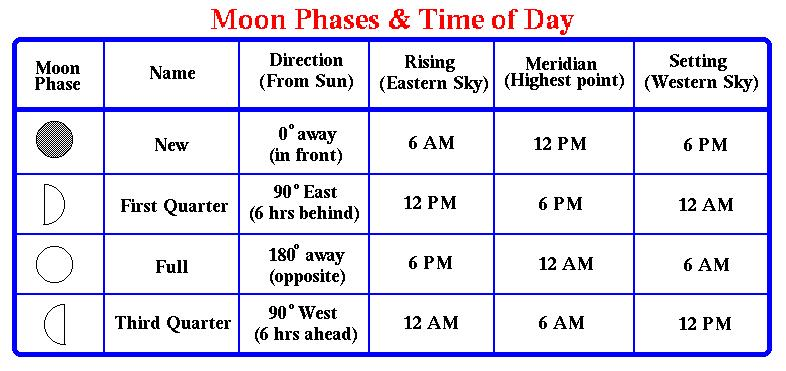
\includegraphics[width=0.7\textwidth]{moon_phases.jpg}
\end{figure}

\subsubsection{Eclipses}
Eclipses occur when the Sun, Moon, and Earth are aligned. A {\bf lunar eclipse} occurs when the Earth lies between the other two, such that the Earth's shadow falls on and blacks out the Moon. A {\bf solar eclipse} occurs when the Moon lies between the Sun and the Earth, so that the Moon block's our view of the Sun (ie. its shadow falls on us).

Since the Moon's orbit is slightly (5 degrees) inclined, eclipses do not happen each month. Eclipses, then, only occur when the Moon passes through the ecliptic; the two locations in which it does are referred to as the {\bf nodes} of its orbit. These times are called {\bf eclipse seasons}, and occur twice per year.

A lunar eclipse occurs when a full moon occurs near a node, a solar eclipse occurs when a new moon occurs near a node.

Since the Moon's shadow has both an {\bf umbra} -- the central area which completely blocks sunlight -- and a {\bf penumbra} -- which only partially blocks sunlight -- these eclipse can look extremely different. If the three objects line up perfectly, we can have a {\bf total lunar eclipse}, in which the Moon is completely blocked during the period of {\bf totality}. More likely is a {\bf partial eclipse}, which only hides a portion of the Moon. Finally, we have {\bf penumbral lunar eclipses}, which shade the Moon but do not completely blot it out.

During totality, the Moon is completely dark for typically less than an hour, save for the red ring around it formed because Earth's atmosphere bends some of the Sun's light toward the Moon (and, to a far lesser extent, due to {\bf gravitational lensing}).

Similarly, we have total and partial solar eclipses based on whether you are within the Moon's umbra or penumbra. When the Moon is too far away for its umbra to even reach the Earth, we see an {\bf annular eclipse}: a ring of sunlight surrounding the Moon when we are directly behind the umbra; otherwise, we see a partial eclipse.

Since the umbra moves across the Earth at a speed of $1,700$ km/h, an eclipse can last no more than a few minutes for any given location on Earth.

The location of the nodes in the Moon's orbit slowly change over time. This gives us an eclipse cycle of 18 years 11.3 days; we call this the {\bf Saros Cycle}. Of course, this only tells us when eclipses will occur, not where they will be visible from on Earth or whether they will be total or partial.

\subsection{Planets}
We can see five planets with the naked eye: Mercury, Venus, Mars, Jupiter, and Saturn. Mercury is rarely visiable, and only near sunrise or sunset. Venus can often be seen shining brightly in the evening (in the West) or before dawn (in the East). Jupiter, when visible, is the brightest star at night. Mars is often recognizeable by its red hue. Saturn has no distinguishing features, but can be identified with star charts.

Planets have different paths of motion that do stars, which is why the word for planet in Greek means ``wandering star''. The planets usually move Eastward through constellations, but sometimes go through periods of {\bf apparent retrograde motion} for anywhere between a few weeks and a few months. This retrograde motion occurs when the Earth ``passes'' the other planet, ie. when their orbits are in line with the Sun.

{\bf Stellar parallax} is the phenomenon of stars appearing to move at different rates given different angles; given the extremely great distances between us and the stars, this is not detectable by the human eye -- though it can be detected by telescopes.
